\documentclass[border=10pt]{standalone}
\usepackage{pgfplots}
\pgfplotsset{compat=1.16}
\begin{document}
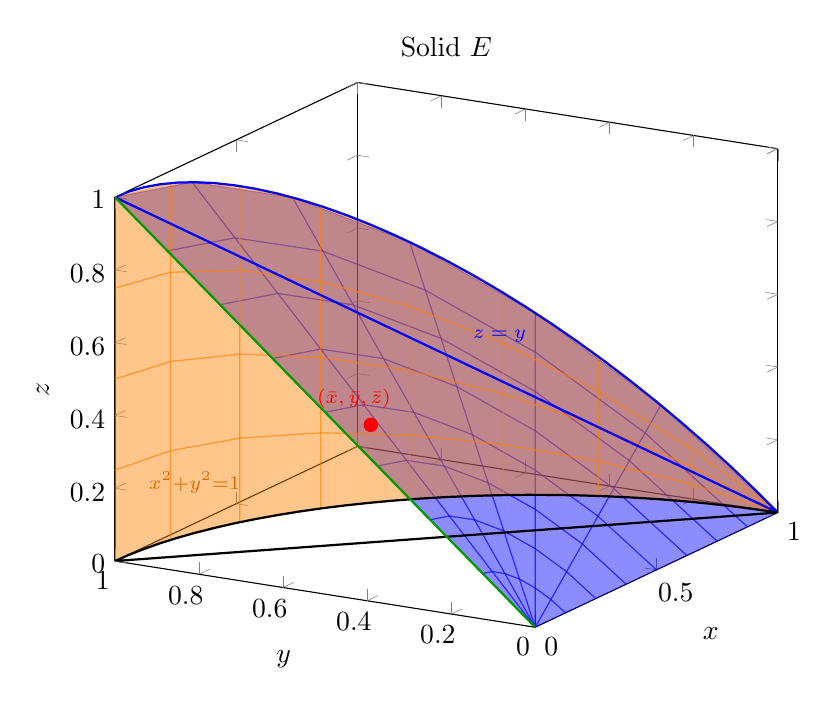
\begin{tikzpicture}
\begin{axis}[
    width=10cm, height=8.5cm, view={-60}{20},
    xmin=0, xmax=1, ymin=0, ymax=1, zmin=0, zmax=1,
    xlabel={$x$}, ylabel={$y$}, zlabel={$z$},
    title={Solid $E$}, every title/.style={font=\small}]
  \addplot3[surf, domain=0:1, y domain=0:90, samples=9, samples y=7,
            blue, opacity=.45, shader=flat] ({x*cos(y)},{x*sin(y)},{x*sin(y)});
  \addplot3[surf, domain=0:90, y domain=0:1, samples=9, samples y=5,
            orange, opacity=.45, shader=flat] ({cos(x)},{sin(x)},{y*sin(x)});
  \addplot3[blue, thick, domain=0:90, samples=30] ({cos(x)},{sin(x)},{sin(x)});
  \addplot3[black, thick, domain=0:90, samples=30] ({cos(x)},{sin(x)},{0});
  \addplot3[green!60!black, thick, domain=0:1, samples=5] (0,{x},{x});
  \addplot3[only marks, mark=*, mark size=2.4pt, red] coordinates {(0.387413,0.615012,0.322264)};
  \node[red, font=\scriptsize] at (axis cs:0.50,0.72,0.34) {$(\bar{x},\bar{y},\bar{z})$};
  \node[blue, font=\scriptsize] at (axis cs:0.20,0.20,0.70) {$z=y$};
  \node[orange!85!black, font=\scriptsize] at (axis cs:0.12,0.88,0.20) {$x^2{+}y^2{=}1$};
\end{axis}
\end{tikzpicture}
\end{document}
